% Circumscribed Parallelepiped
% Author: Axel Pavillet
\documentclass[tikz,border=0pt]{standalone}
\usepackage{tkz-graph}
\usepackage{relsize}
\usepackage{adjustbox}
\usetikzlibrary{fit,arrows,decorations.markings,calc,shapes,backgrounds}

\definecolor{cd40000}{RGB}{212,0,0}
\definecolor{cffffff}{RGB}{255,255,255}
\definecolor{c2a7fff}{RGB}{42,127,255}
\definecolor{c0000d9}{RGB}{0,0,217}
\definecolor{c0000ff}{RGB}{0,0,255}
%\definecolor{bluecolor}{RGB}{71,190,255}
%\definecolor{bluecolor}{RGB}{255,186,81}
\definecolor{bluecolor}{RGB}{136,224,223}
\definecolor{darkgrey}{RGB}{150,150,150}
\definecolor{lightgrey}{RGB}{226,226,226}

\colorlet{Rcolor}{bluecolor}

\usepackage{relsize}

\begin{document}
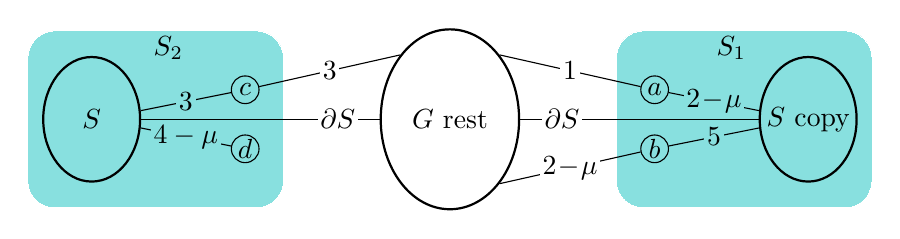
\begin{tikzpicture}[scale=0.5,yscale=0.5,xscale=1.3]

\draw[color=white,rounded corners=10pt,line width=0pt,fill=Rcolor] (3.25,-4.5) rectangle ++(5,9);
\draw[color=white,rounded corners=10pt,line width=0pt,fill=Rcolor] (-3.25,-4.5) rectangle ++(-5,9);


\begin{scope}[every node/.style={draw,ellipse,minimum width=50, minimum height=65,inner sep=0pt,fill=none,thick}]
\node (G) at (0,0) {$G$ rest};
\end{scope}
\begin{scope}[every node/.style={draw,ellipse,minimum width=35,minimum height=45,inner sep=0pt,fill=none,thick}]
\node[text width=10pt, align=center] (S1) at (7,0) {\mbox{$\!\!\!\!\!\!S$ copy}};
\node (S2) at (-7,0) {$S$};
\end{scope}


\node[line width=0] at (5.5,3.6) {$S_1$};
\node[line width=0] at (-5.5,3.6) {$S_2$};

\begin{scope}[every node/.style={draw,minimum width = 10pt,circle,inner sep=0pt,fill=none}]
\node (a) at (4,1.5) {$a$};
\node (b) at (4,-1.5) {$b$};
\node (c) at (-4,1.5) {$c$};
\node (d) at (-4,-1.5) {$d$};
\end{scope}

\begin{scope}[every node/.style={fill=Rcolor,inner sep=1pt}]
  \draw (a) to node[midway, ] {$2\!-\!\mu$} (S1.170);
  \draw (b) to node[midway,  ] {$5$} (S1.190);
  %\draw (d) to node[midway, below, fill=none, ] {$1$} (G.south west);
  \draw (c) to node[midway, ] {$3$} (S2.10);
  \draw (d) to node[midway,  ] {$4-\mu$} (S2.350);
 \end{scope}
\begin{scope}[every node/.style={fill=white,inner sep=1pt}]  
  \draw (b) to node[midway, ] {$2\!-\!\mu$} (G.south east);
  \draw (a) to node[midway, ] {$1$} (G.north east);
 \draw (c) to node[midway,  ] {$3$} (G.north west);
  \draw (S1) to node[pos=0.825 ] {$\partial S$} (G);
  \draw (S2) to node[pos=0.825 ] {$\partial S$} (G);
\end{scope}

% \draw (-7,0) ellipse (1 and 2);
% \draw (7,0) ellipse (1 and 2);
% \draw (3,2) ellipse (0.3 and 0.3);
% \draw (3,-2) ellipse (0.3 and 0.3);
\end{tikzpicture}
\end{document}
